\documentclass{article}
\usepackage[pdfborder={0 0 0}, colorlinks=true]{hyperref}
\usepackage{multicol}
\usepackage{color}
\author{CISC475/675 Spring 2010}

\title{REX User's Manual}
\date{\today}

\begin{document}
\maketitle
\tableofcontents
\newpage

\section{Introduction}
The REX software package was designed as part of the CISC475 course,
to create a solution for Professor Harvey. Professor Harvey wishes to create
multiple versions of each exam for the classes he instructs. However,
this can be very time consuming, and as the number of exams created
increases, the amount of effort needed to be exerted to assure the
accuracy of the exams increases proportionally.

We sought to solve these problems for Professor Harvey, and created the
REX software as an educational exercise in real-world software
development practices.

The REX software runs without any installation requirements beyond the
need of an appropriate Java VirtualMachine. The REX software will take
UEF File and an ECF File as input, and non-deterministically save
some number of exam files and answer key files in a desired directory.

\section{Overview}
The Rex 

\section{Installation}
The REX software does not require any installation. It is suggested to
place the \texttt{rex.jar} executable in a directory within the user
path on UNIX systems, but this is not necessary for proper operation
of the software.

While REX does not require an installer or any unpacking of it's software,
there must be a version of the Java Runtime Environment installed. The
following list of system requirements must be met in order to run REX.

\subsection{Minimum System Requirements}
\begin{itemize}
\item Java Runtime Environment (JRE) 1.6: 

Available at 
\verb|http://java.sun.com/javase/downloads|
% do we need memory requirements? like a 1G of ram? -Haley
\end{itemize}

\subsection{Building From Source}



\section{Universal Exam File (UEF)}

Please see Figure \ref{fig:SampleUEF} on page \pageref{fig:SampleUEF} for 
an example Universal Exam File.

\section{Exam Configuration File (ECF)}
The ECF file is a text file with a \texttt{.tex} extension that consists
of a series of constraints. Each constraint is separated by a semicolon,
with comments being all text that follows after a pound symbol 
(\texttt{\#}) until the end of the line. Please see Figure \ref{fig:SampleECF} 
on page \pageref{fig:SampleECF} for an example Exam Configuration File.

There are four defined commands for the ECF file.

\subsection{Group Constraints}
A group constraint is a command of the form \texttt{include \textcolor{blue}{int count}
problems on \textcolor{blue}{string topic} with difficulty in \textcolor{blue}{interval\footnote{An interval is a pair of decimals separated by two periods, in between a pair of braces or parenthesis. A brace on an end indicates that edge is inclusive, and a parenthesis that the edge is exclusive. For example, \texttt{[3..5)} would be the range from 3 to 5, including 3 but not including 5.} difficulty} at \textcolor{blue}{int points} points;}.

The command will choose \textcolor{blue}{count} problems from \textcolor{blue}{topic} that fall in the \textcolor{blue}{difficulty} range, and assigns all of them \textcolor{blue}{points} points.

For overlapping constraints, REX will attempt find the largest set of questions that resolves all constraints. That is, if there exist two identical constraints for 5 problems each, REX will attempt to find 10 questions total. If REX cannot accomplish this, the request will result in an \hyperref[RexUnsatisfiableException]{RexUnsatisfiableException}. 

\subsection{Required Problem Constraints}
A required problem constraint is a command of the form \texttt{includeall \textcolor{blue}{string label} at \textcolor{blue}{int points} points;}.

This will ensure the the question with the \textcolor{blue}{label} given is included in every
generated exam, and will be given \textcolor{blue}{points} points. 

Multiple \textcolor{blue}{label}'s can be given in one command by separating them by commas. This will have the same effect as if each label was given on its own line.

\subsection{Append Text}
An append text command is a command of the form \texttt{append \textcolor{blue}{string label};}

This will take the text contained in the block with the given \textcolor{blue}{label}, and append it to the end of the exam.

\subsection{Version Definition}
A version definition of a command of the form \texttt{versions are \textcolor{blue}{string versions};}

\textcolor{blue}{Versions} are a list of strings, separated by commas, used to distinguish the different exams generated. Each generated exam will use one item in the list, and so there must be at least as many items as there will be exams generated. 

In the UEF file, you can use the \textbackslash{examversion} command to insert the current version string. One example use for this is to have a different date format for each generated exam, so that the exams can be easily distinguished from one another, but a naive student would not know how to tell if his neighbor has a similar exam.

\section{Usage}
After creating a UEF and ECF file \texttt{rex input.uef input.ecf}.  REX will parse the contents of the UEF and ECF and generate the appropriate number of output exams, as specified in the ECF file.

Please see the following sections for information on UEF and ECF content format.

\section{Troubleshooting}
Because of the requirements that REX places upon the input it parses, REX may present the user with a variety of errors. Additionally, it's possible that REX might process the request without any errors or warnings, but will provide an undesired output.

\subsection{Errors}
\subsubsection{RexParseException}
This error means that REX encountered a syntactic error in either the UEF or ECF file. Please consult the provided error message for more information.

\subsubsection{RexUnsatisfiableException}
\label{RexUnsatisfiableException}
This error means that the input files were parsed correctly, but that
REX determined that the requirements from the ECF cannot be resolved
using the provided UEF file. Generally, this means that there aren't
enough problems in the UEF. Either reduce the number of requested
problems in the ECF, or create new problems in the UEF to resolve
this error.

Note: REX resolves the requirements in the ECF simultaneously. This means
that if the ECF has two identical requirements of 5 questions each, REX
will require at least 10 satisfactory questions.



% How do we add color to this to make it easier
% to read? -Haley

% We can add color by using \textcolor{declared-color}{text} - BUT, we can't put that in a verbatim.
% We'd have to escape all the LaTeX commands to use that. We'd have to at the least place a 
% \textbackslash for ever instance of a backslash - \begin, \section, etc.
% Also, I can't find an easy way to make a long section of text appear teletype other than
% using \begin{verbatim}.
\begin{figure}
\begin{verbatim}
    \documentclass{exam} 
    \usepackage{fullpage}
    \usepackage{amsmath}
    \usepackage{comment}
    \usepackage{graphicx}

    \begin{document}

    \examheader{CISC 106}{UEF Example}{Developed: 2010}

    \section{Topic}

    \begin{block}{FSA Description}
      In the following four problems, let $A$ denote a finite-state
      automaton with exactly one accepting state.
    \end{block}

    \begin{problem}{topic}{15}
      This is a problem
      \begin{answers}
        \answer This is an answer that is not correct
        \answer answer
        \answer[fixed] This is a fixed answer that is not correct
        \answer[correct] This is a correct answer
        \answer answer
        \answer[fixed,correct] fixed correct answer
      \end{answers}
    \end{problem}

    \begin{figure}[placement h]
      \begin{center}
          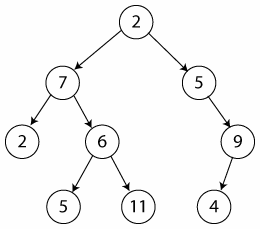
\includegraphics[scale=0.50]{binary_tree.png}
          \caption{Traverse Binary Tree}
          \label{fig:binary tree}
      \end{center}
    \end{figure}

    \begin{block}{Goodbye Message}
      Did you remember to write your name on the first page?  Did you
      attempt to answer every question?    Have a good holiday.
    \end{block}

    \end{document}
\end{verbatim}
\caption{Sample UEF.txt}
\label{fig:SampleUEF}
\end{figure}

\begin{figure}
\begin{verbatim}
include 5 problems on "Finite State Automata" with difficulty in [0,20)
  at 3 points;
include 5 problems on "ssort" with difficulty in [20,\infty) at 2 points;
include 3 problems on "arithmetic" with difficulty in [0,10] at 1 points;
include 3 problems on "arithmetic" with difficulty in (-\infty,\infty) at 3 points;

# the following problems will be included in their corresponding
# sections on any generated exam
includeall prob:arithmetic:prime, prob:arithmetic:composite, prob:misc:hat,
  prob:misc:complexity at 5 points;

append "Goodbye Message"; # this block will be added at end

versions are "1/21/2010", "Jan.\ 21, 2010", "21-jan-2010", "JAN.\ 21 2010";
\end{verbatim}
\caption{Sample ECF.ecf}
\label{fig:SampleECF}
\end{figure}

\end{document}
